\documentclass{jsarticle}
\usepackage[dvipdfmx]{graphicx}
\title{第17回全国高等専門学校帰宅選手権(仮)}

\begin{document}

\section{どんなゲーム?}\label{ux3069ux3093ux306aux30b2ux30fcux30e0}

相手の帰宅途中に地雷を設置して相手の帰宅を妨げつつ、
自分は相手の妨害を乗り越えて帰り着くことが目的です。

ただし、帰宅途中に諦めるという選択もあります。このさいは途中までのポイントがもらえます。

最終的にはポイントの多い方が勝ちとなります。

プレイ時間はどれだけ考えるかに左右されますが、3分以上を見越してください。

\section{画面名称と遷移}\label{ux753bux9762ux540dux79f0ux3068ux9077ux79fb}

\begin{figure}[htbp]
\centering
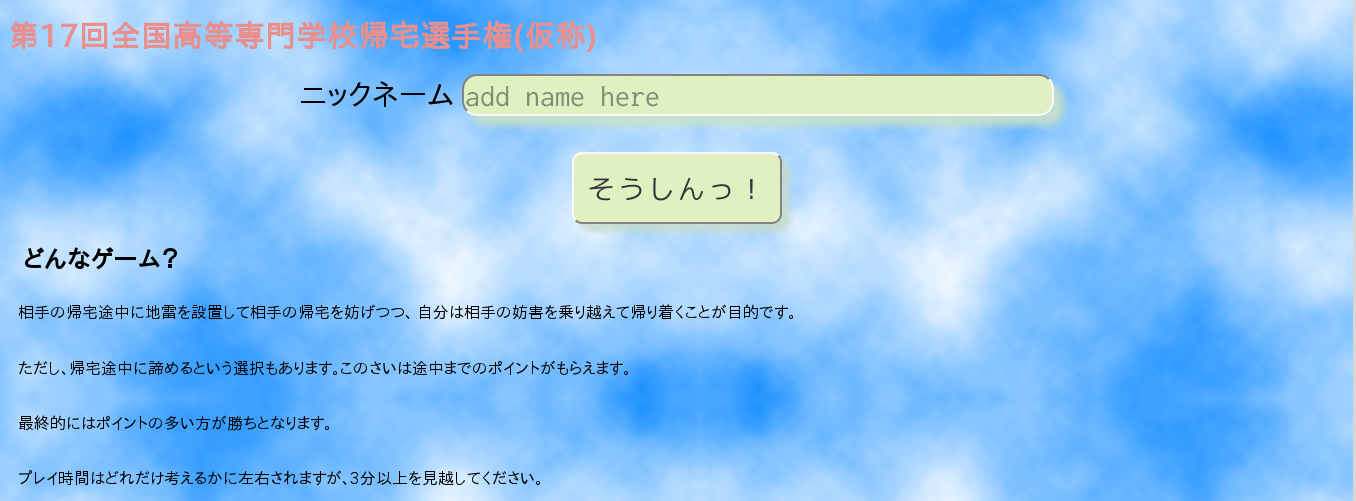
\includegraphics[width=10cm]{./top.png}
\caption{トップ画面}
\end{figure}

ここでニックネームを入力することで入室します。

\begin{figure}[htbp]
\centering
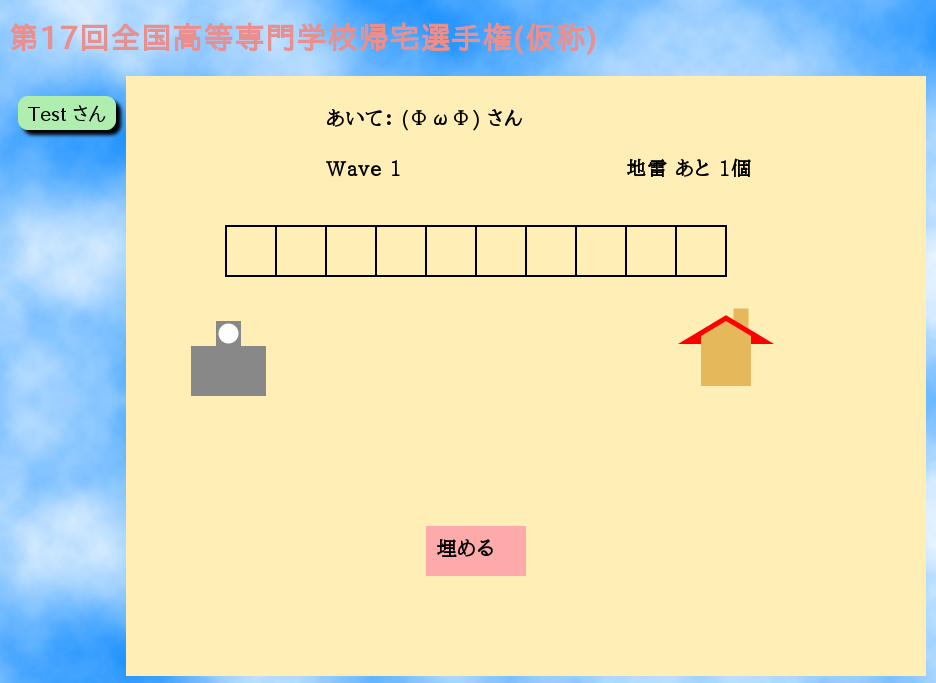
\includegraphics[width=10cm]{./mine.png}
\caption{地雷敷設画面}
\end{figure}

ここで相手の帰宅路に地雷を埋めます。

\begin{figure}[htbp]
\centering
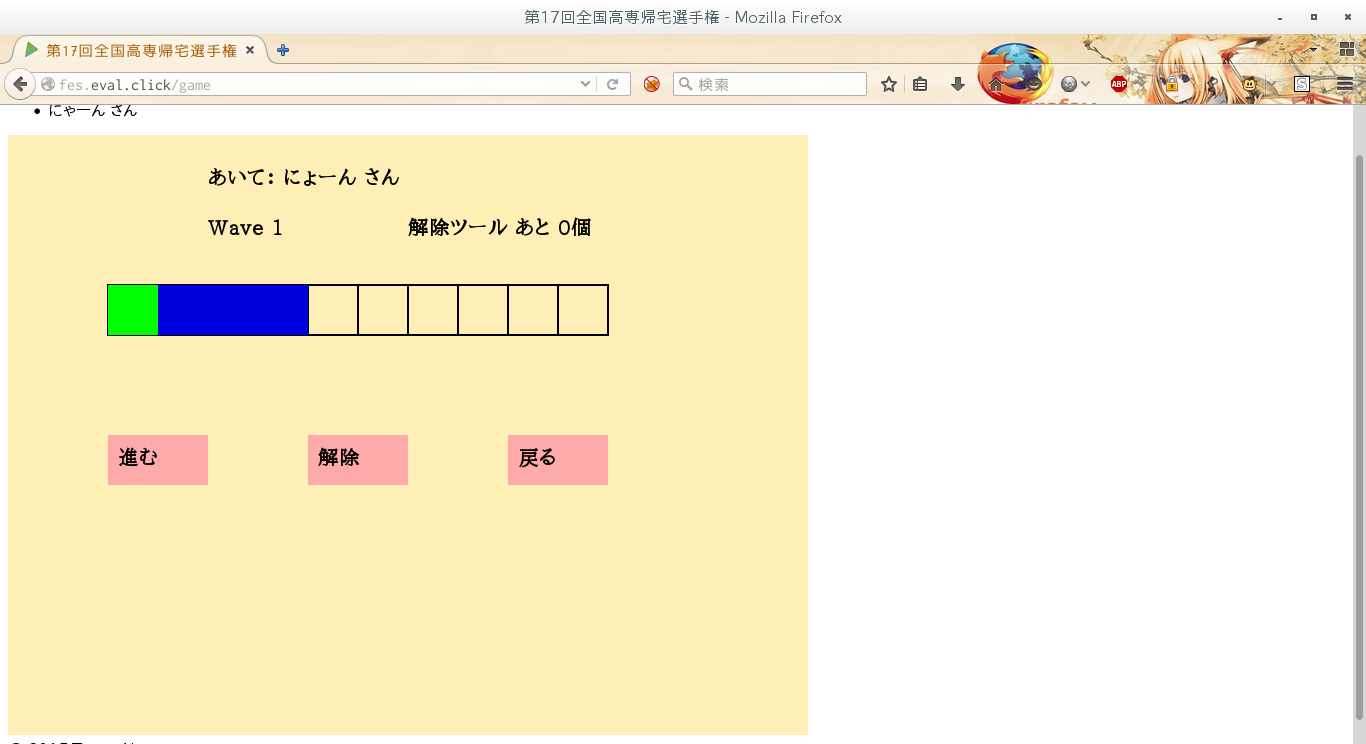
\includegraphics[width=10cm]{./do.png}
\caption{帰宅画面}
\end{figure}

ここで実際に帰り着くよう試みます。

ツールをうまく使いながら帰ってください。
諦める場合は戻るをクリックしてください。

\begin{figure}[htbp]
\centering
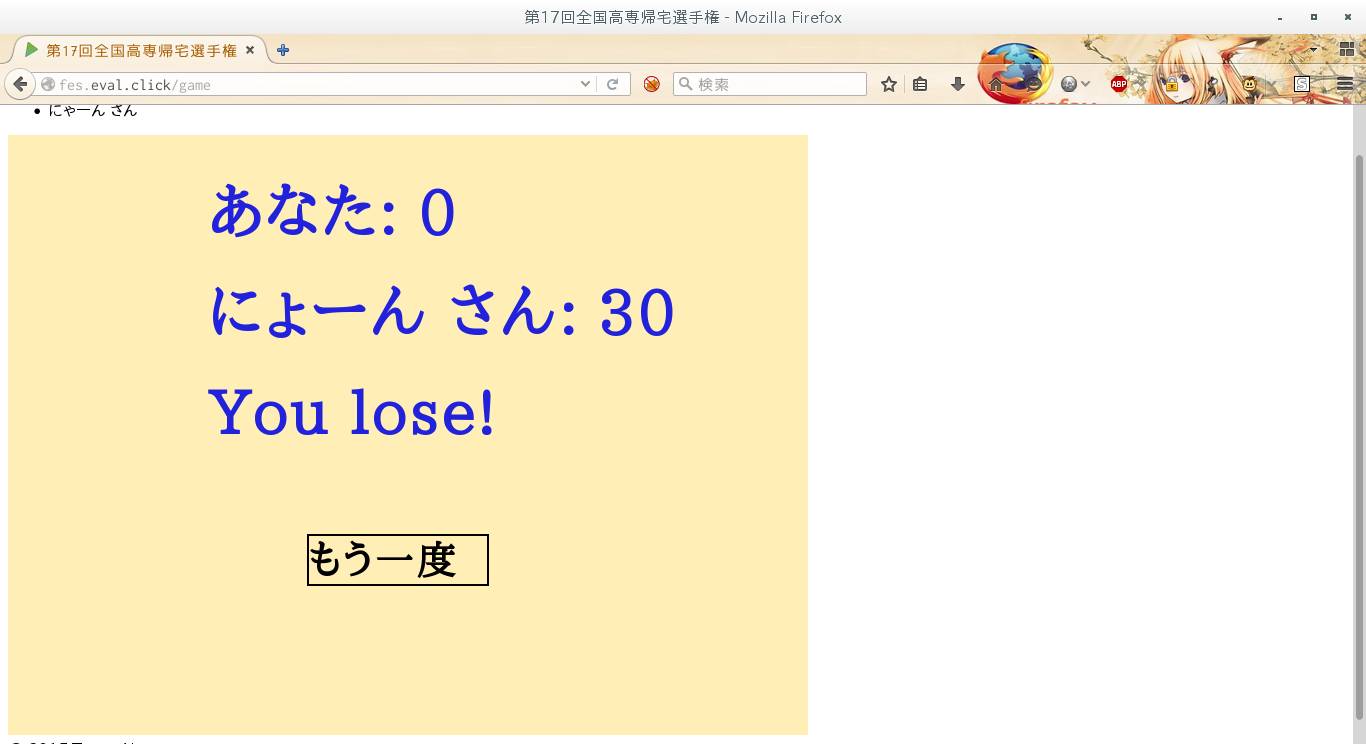
\includegraphics[width=10cm]{./result.png}
\caption{最終結果}
\end{figure}

ゲームの結果が表示されます。

もう一度を押しても同じ相手とマッチングされるとは限りません。

\section{操作方法}\label{ux64cdux4f5cux65b9ux6cd5}

\subsection{トップ画面}\label{ux30c8ux30c3ux30d7ux753bux9762}

\begin{figure}[htbp]
\centering
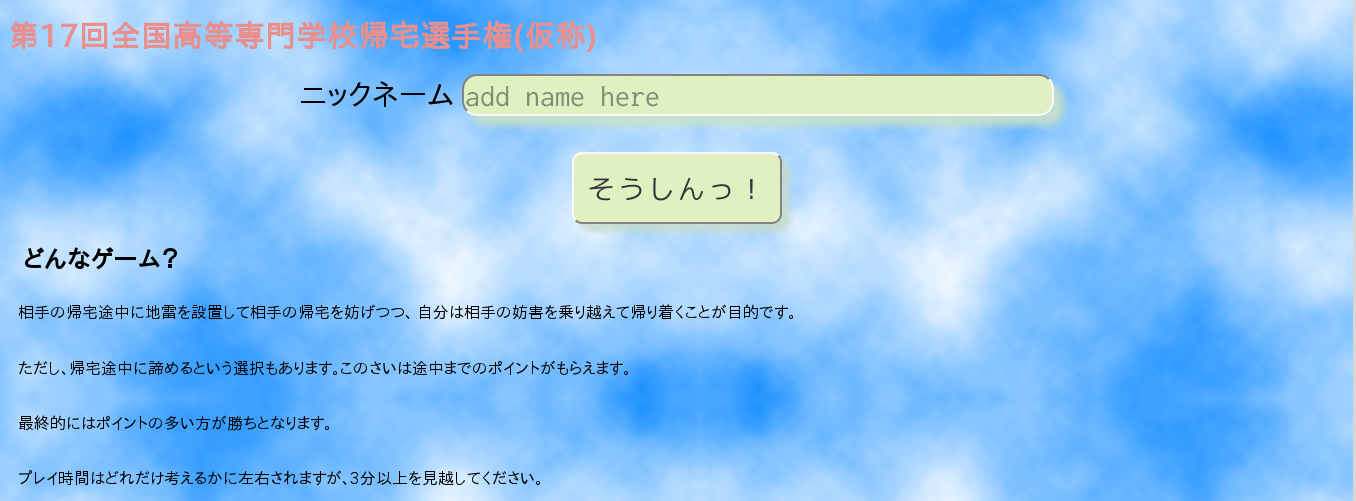
\includegraphics[width=10cm]{./top.png}
\caption{トップ画面}
\end{figure}

テキストボックスにニックネームを入れて「そうしんっ!」と書かれているボタンをクリックするか、
Enterキーを入力してください。

ゲーム本体のページに遷移しますが、その際ニックネームが見つからない場合はエラーが返ってくるか、
トップページが再び表示されるかします。その場合はもう一度やってみてください。

\subsection{地雷敷設画面}\label{ux5730ux96f7ux6577ux8a2dux753bux9762}

\begin{figure}[htbp]
\centering
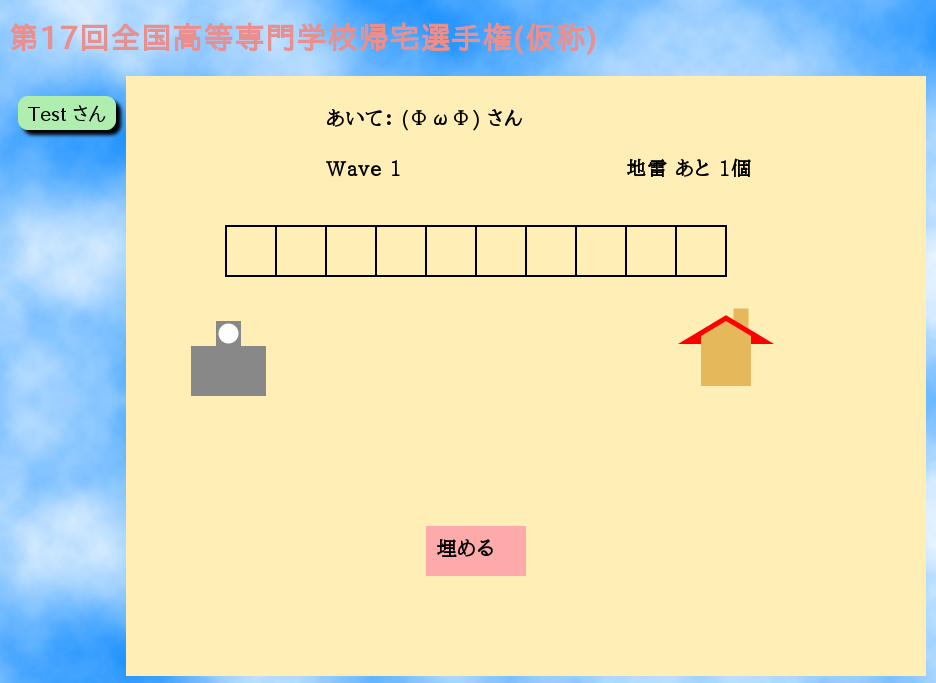
\includegraphics[width=10cm]{./mine.png}
\caption{地雷敷設画面}
\end{figure}

画面上のますをクリックすることで地雷を埋める/埋めないをトグルします。満足したら埋める
のところをクリックしてください。

クリックするまではサーバーにデータが送られることはありません。

自分がデータを送ったあとでも、相手のデータが来ない限りは通信待機画面になります。

\subsection{帰宅画面}\label{ux5e30ux5b85ux753bux9762}

\begin{figure}[htbp]
\centering
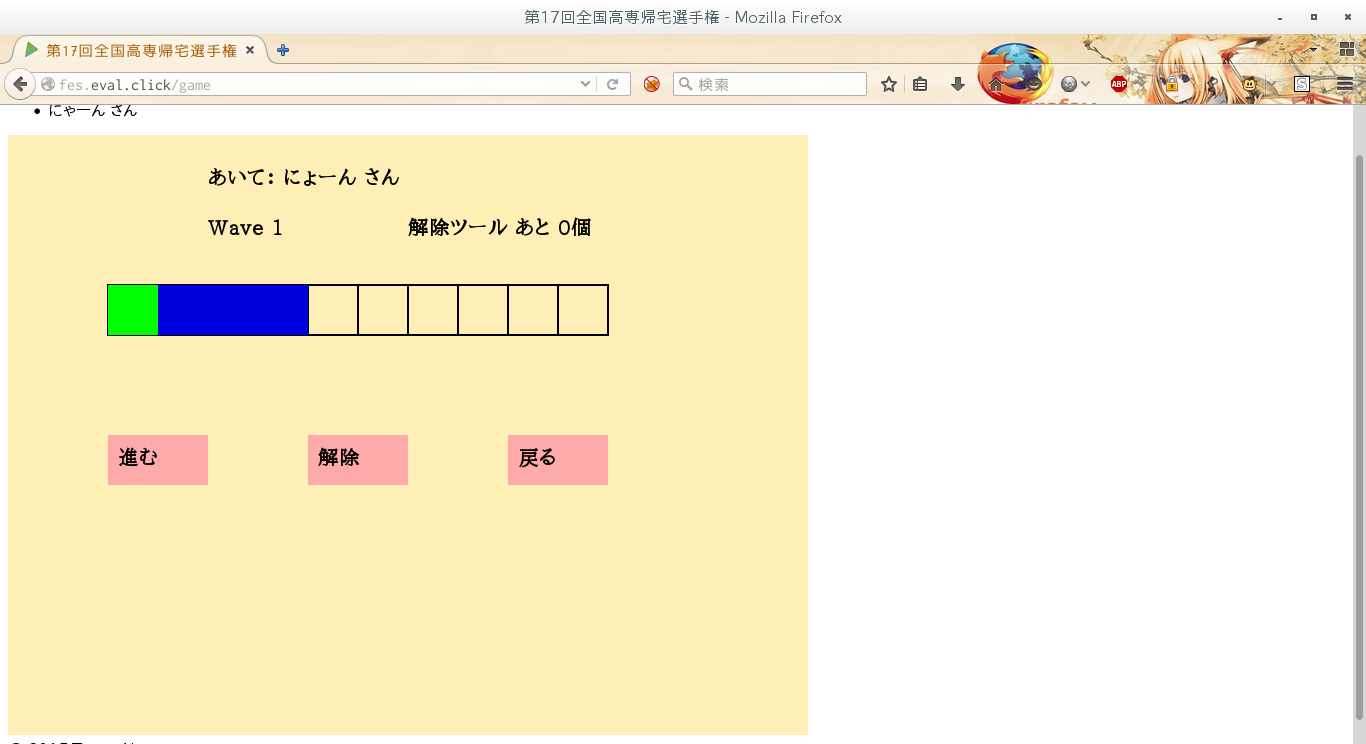
\includegraphics[width=10cm]{./do.png}
\caption{帰宅画面}
\end{figure}

進むはただただ進みます。解除はツールを使用して解除する動作を行った後に一歩進みます。
ツールは解除した、しないにかかわらず数が減るので、戦略的に使用してください。

戻るは諦めて学校に戻ります。この場合得点はその時点まで進んだマスと同等になります。

すべてのマスが緑か蒼になるとウェーブクリアで、結果が送られます。

途中で地雷を踏んでしまった場合は得点は0となります。(以前のウェーブの得点が消えるわけではありません。)

\subsection{最終結果}\label{ux6700ux7d42ux7d50ux679c}

\begin{figure}[htbp]
\centering
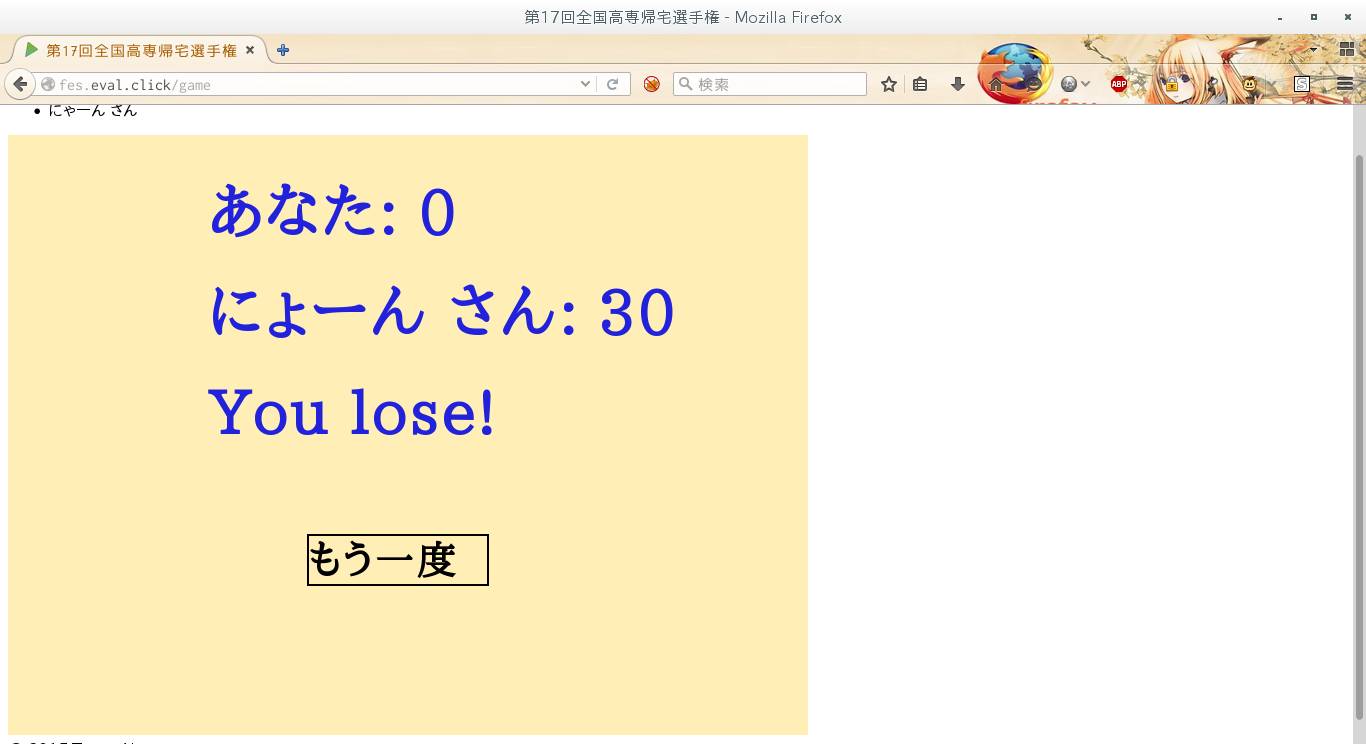
\includegraphics[width=10cm]{./result.png}
\caption{最終結果}
\end{figure}

このゲームの最終結果の画面です。
相手の名前と得点。自分の得点と勝敗が表示されます。

もう一度をクリックするとゲームの初期状態になり、またマッチング待ちとなります。

\section{既知の問題など}\label{ux65e2ux77e5ux306eux554fux984cux306aux3069}

\begin{itemize}
\item  
  進むを連打するとまれに通信待機中のままかたまってしまう場合があります。 対策としてはゆっくりプレイすることを推奨します。
\item
  見た目が\ldots{}\ldots{} 仕様です
\item
  見た目が!! 仕様ですっ!! 誰だっ! 技術屋にデザインを期待した奴はっ!
\end{itemize}

\section{使用技術}\label{ux4f7fux7528ux6280ux8853}

\subsection{言語}\label{ux8a00ux8a9e}

\begin{itemize}
\item
  Server: Scala
\item
  Client: Javascript
\end{itemize}

\subsection{その他}\label{ux305dux306eux4ed6}

\begin{itemize}
\item
  Akka
\item
  Websocket
\item
  Playframework
\item
  HTML5 Canvas
\end{itemize}

\section{作者情報等}\label{ux4f5cux8005ux60c5ux5831ux7b49}

\begin{itemize}
\item
  4Jの誰かと4Jの誰かと\ldots{}
\item
  作った奴しか答えられない場合があります
\end{itemize}

\end{document}
